\documentclass[10pt]{beamer}

\usetheme{Montpellier}
\usecolortheme{beaver}

\usepackage{lmodern}
\usepackage{mathtools}
\usepackage{amsmath}
\usepackage{listings}
\usepackage{mdframed}
\usepackage{xcolor}
\usepackage{parskip}
\usepackage{substr}
\usepackage{hyperref}
\usepackage{etoolbox}
\usepackage{tipa}
\usepackage{pdfpages}
\usepackage{multicol}
\usepackage{cprotect}
\usepackage{booktabs}
\usepackage{silence}
\usepackage[backend=biber, style=ieee]{biblatex}
\usepackage[english,ngerman]{babel}
\usepackage{csquotes}
%\hypersetup{colorlinks = true, urlcolor=blue, linkcolor=white}
\mode<presentation>{}
\beamertemplatenavigationsymbolsempty
\setbeamertemplate{footline}[frame number]
\setbeamercolor{title in head/foot}{fg=black}
\setbeamercolor{subsection in head/foot}{fg=black}



\WarningFilter{biblatex}{Patching footnotes failed}

\renewcommand*{\bibfont}{\tiny}

\bibliography{resources.bib}

\titlegraphic{
\includegraphics[keepaspectratio, height=0.15\textheight]{img/logo_hertie.png} \\ [1em] 
\includegraphics[keepaspectratio, height=0.1\textheight]{img/logo.png}}

\title{\textbf{MEA Analysis Toolbox}}
\author{\vspace{-0.7cm}F. Klopfer}
\date{\today}

\begin{document}
\frame{\titlepage}
\section{Task}
\begin{frame}{Task}
\begin{itemize}
 \item Task: Detect peaks, seizure-like bursts \& characterize them. \\
    Provide GUI. \\ [1em]
 \item Contraints: \begin{itemize}
                    \item many channels \\ [1em]
                    \item high sampling rate \\ [1em]
                    \item high heterogeneity (slices) \\ [2em]
                   \end{itemize}
  \item Existing toolboxes are
  \begin{itemize}
   \item proprietary or vendor specific
   \item quality-wise insufficient
  \end{itemize}
\end{itemize}
\end{frame}

\section{What's there}
\begin{frame}
\begin{center}
 \begin{Huge}
  \textbf{What's there}
 \end{Huge}
 \end{center}
\end{frame}

\begin{frame}{So far...}
  What is there so far  \vspace{0.5em}
  \begin{itemize}
    \item was developed in $\approx10$ weeks, \\ [1em]
    \item without recording a single slice myself, \\ [1em]
    \item without analyzing more than 1-2 samples myself, \\ [1em]
    \item without having extensive knowledge about the setup. \\ [2em]
  \end{itemize}
  $\Rightarrow$ that's exactly what will follow in the next 6 months.
\end{frame}

\begin{frame}[allowframebreaks]{MEA Analysis Toolbox}
    Semi-automated data analysis pipeline with UI. \\
   
     Currently supports MultiChannel Systems 256 electrode MEA \\ [1em]
      \begin{center}
        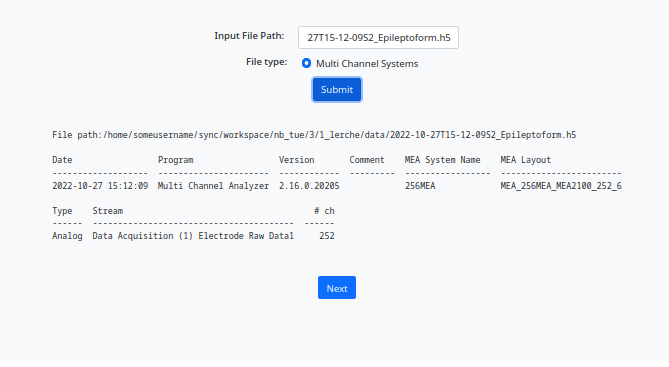
\includegraphics[keepaspectratio,width=0.8\framewidth]{img/4_import.png}
      \end{center}
      \framebreak
      
     Graphical selection of electrodes and time window \\ 
      \begin{center}
        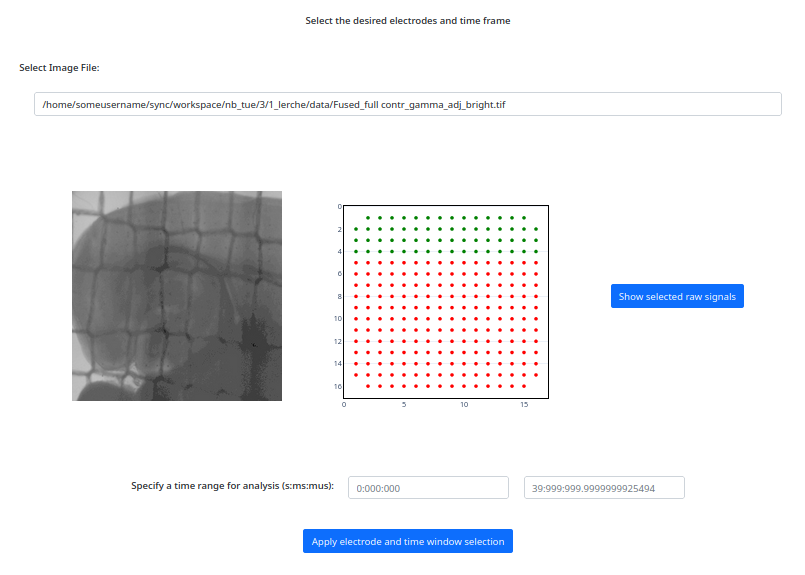
\includegraphics[keepaspectratio,width=0.8\framewidth]{img/4_select.png}
      \end{center}
      \framebreak
      
     Preprocessing: electrical humming, bandpass, bandstop, downsampling \\
      \begin{center}
        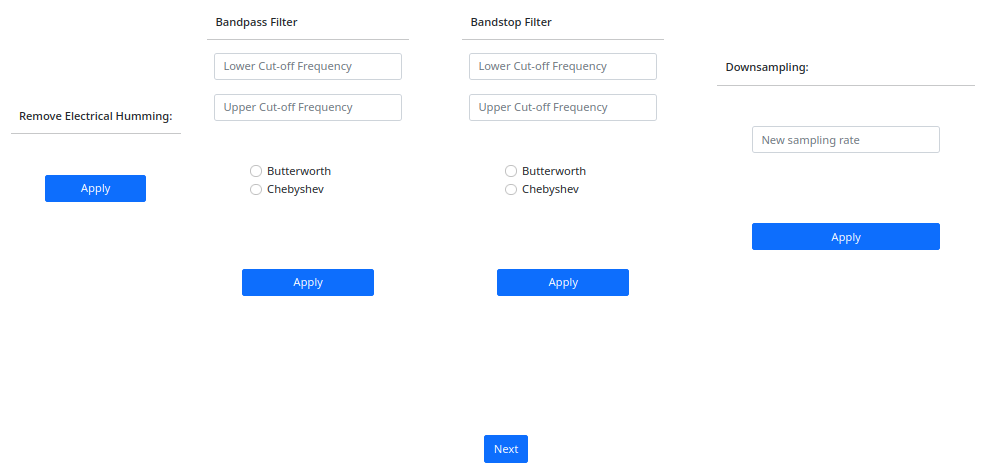
\includegraphics[keepaspectratio,width=0.8\framewidth]{img/4_preproc.png}
      \end{center} 
      \framebreak
      
    Exploration \& Analysis: 
      \begin{center}
      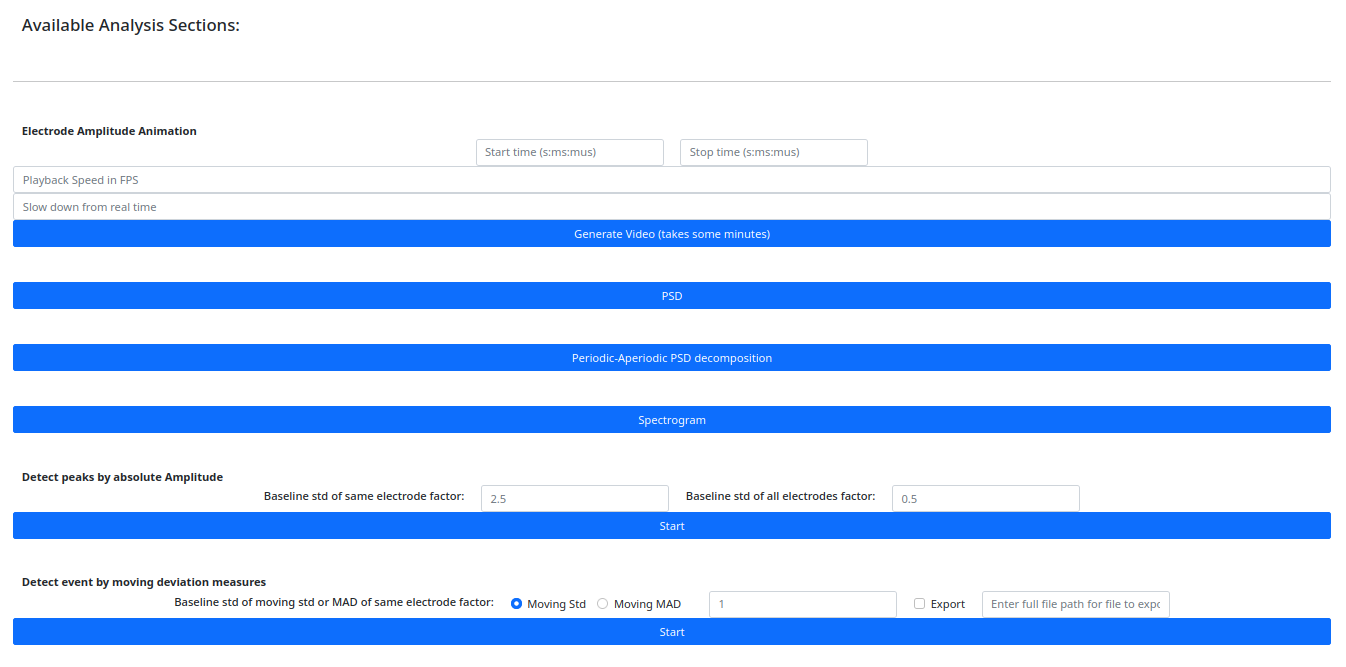
\includegraphics[keepaspectratio,width=0.8\framewidth]{img/4_analyze.png}
      \end{center}
      \framebreak
    Exploration: raw signals, absolute amplitude animation, PSD, spectrogram \\ 
      \begin{center}
        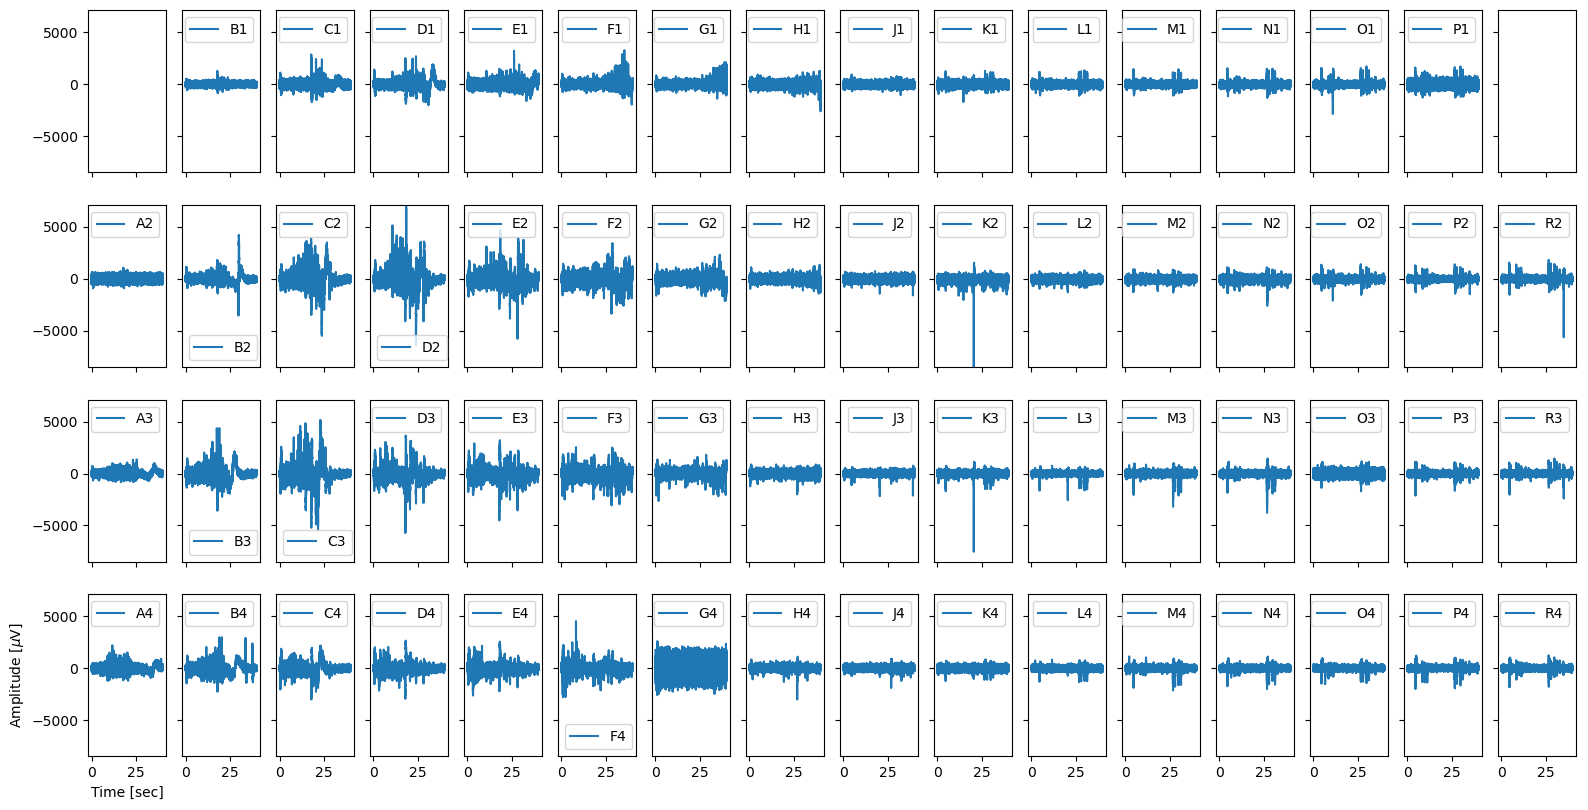
\includegraphics[keepaspectratio,width=0.9\framewidth]{img/4_raw.png}
      \end{center}
      \framebreak
      \begin{center}
        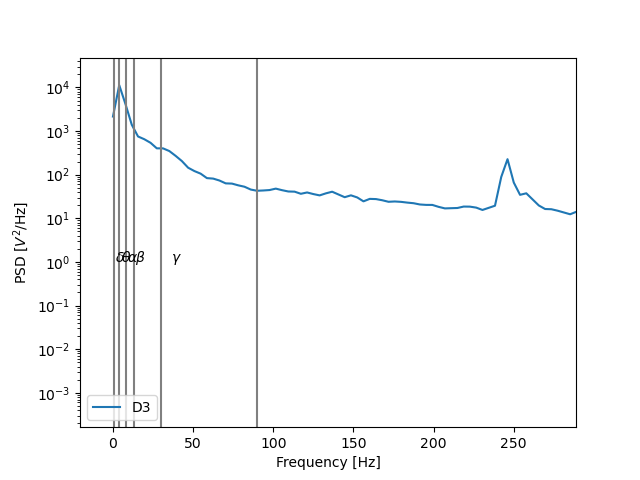
\includegraphics[keepaspectratio,width=0.8\framewidth]{img/4_psd.png}
      \end{center}
      \framebreak
      \begin{center}
        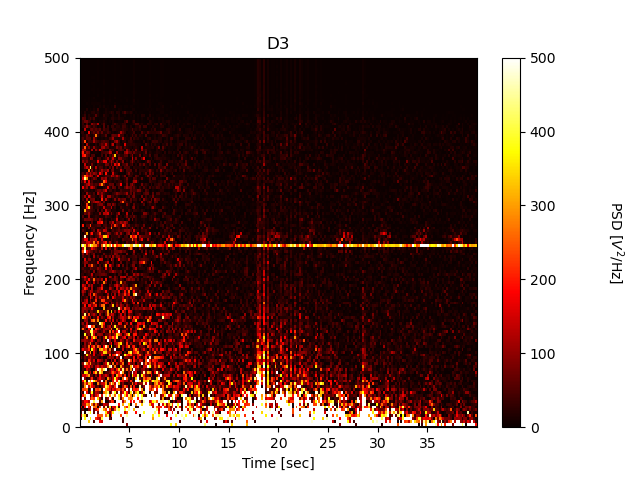
\includegraphics[keepaspectratio,width=0.8\framewidth]{img/4_spectrogram.png}
      \end{center}
      \framebreak
      
     Analysis: Peak detection by threshold based STD per channel, burst detection based on moving STD or moving mean absolute deviation \\
      \begin{center}
       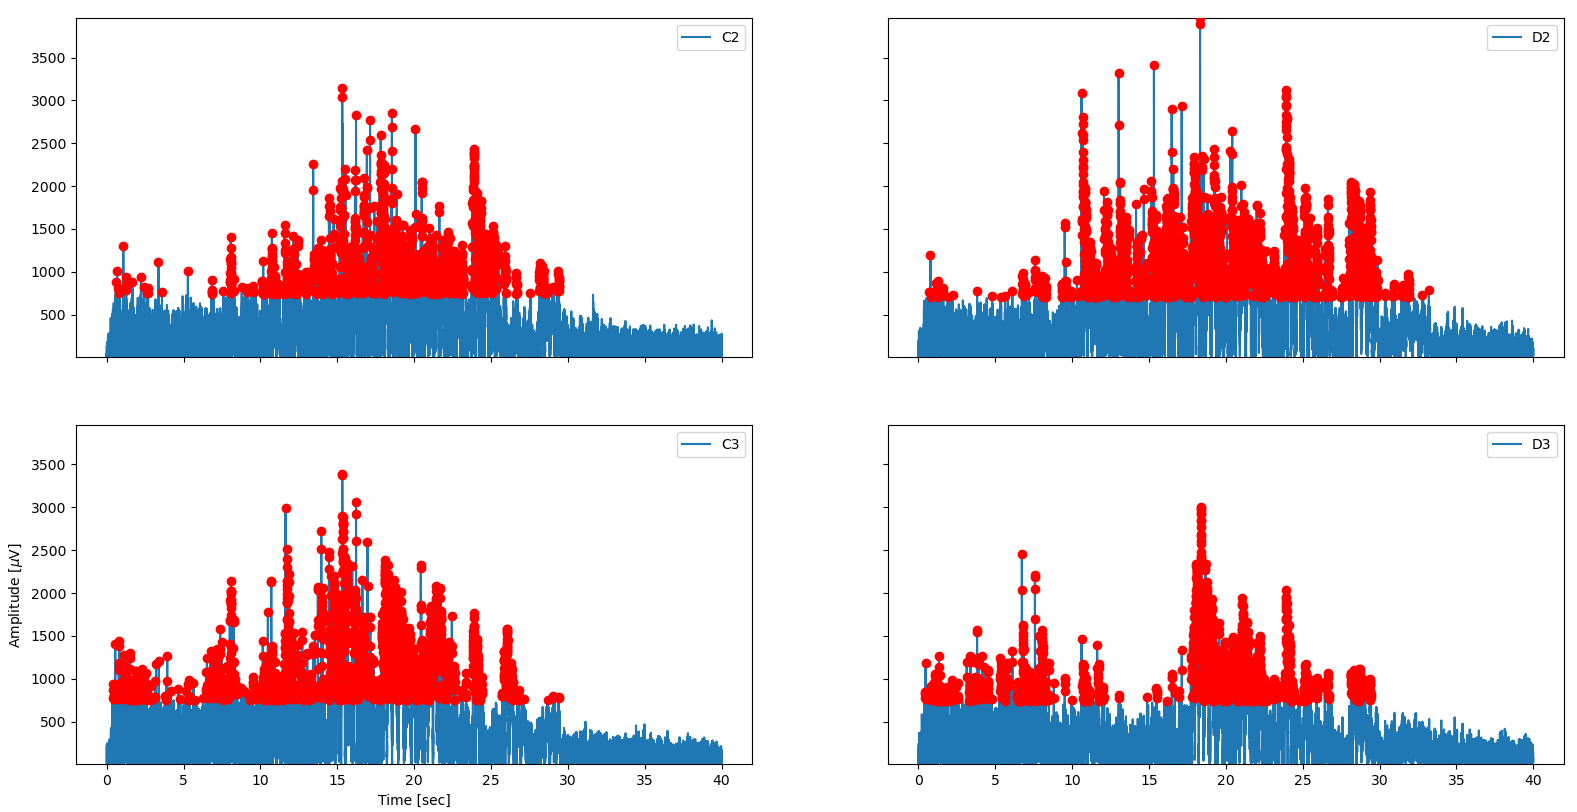
\includegraphics[keepaspectratio,width=\framewidth]{img/4_peaks_amplitude.png}
      \end{center}
      \framebreak
      \begin{center}
      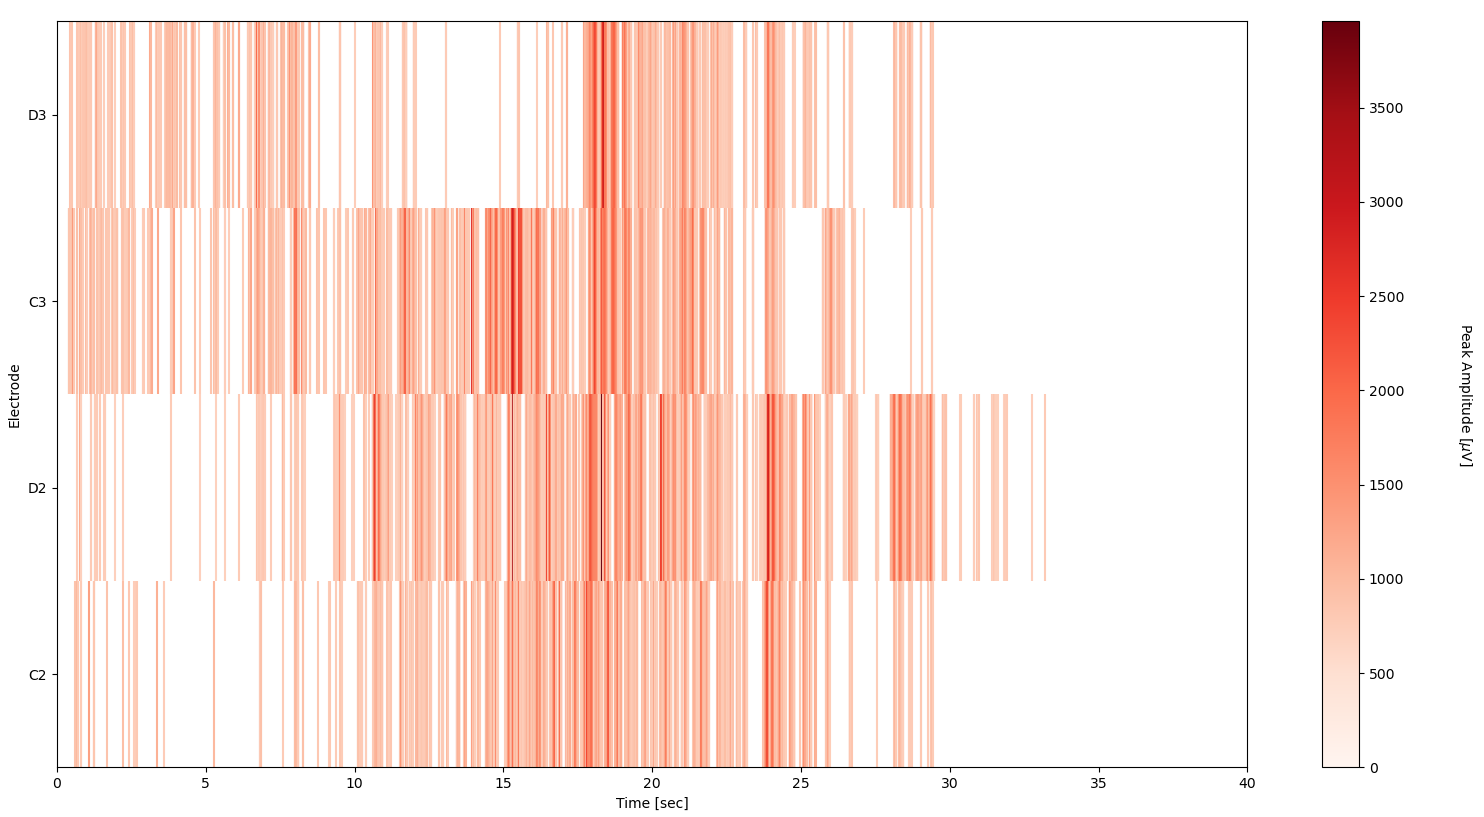
\includegraphics[keepaspectratio,width=\framewidth]{img/4_raster_amplitude.png}
      \end{center}
      \framebreak
      
      \begin{center}
       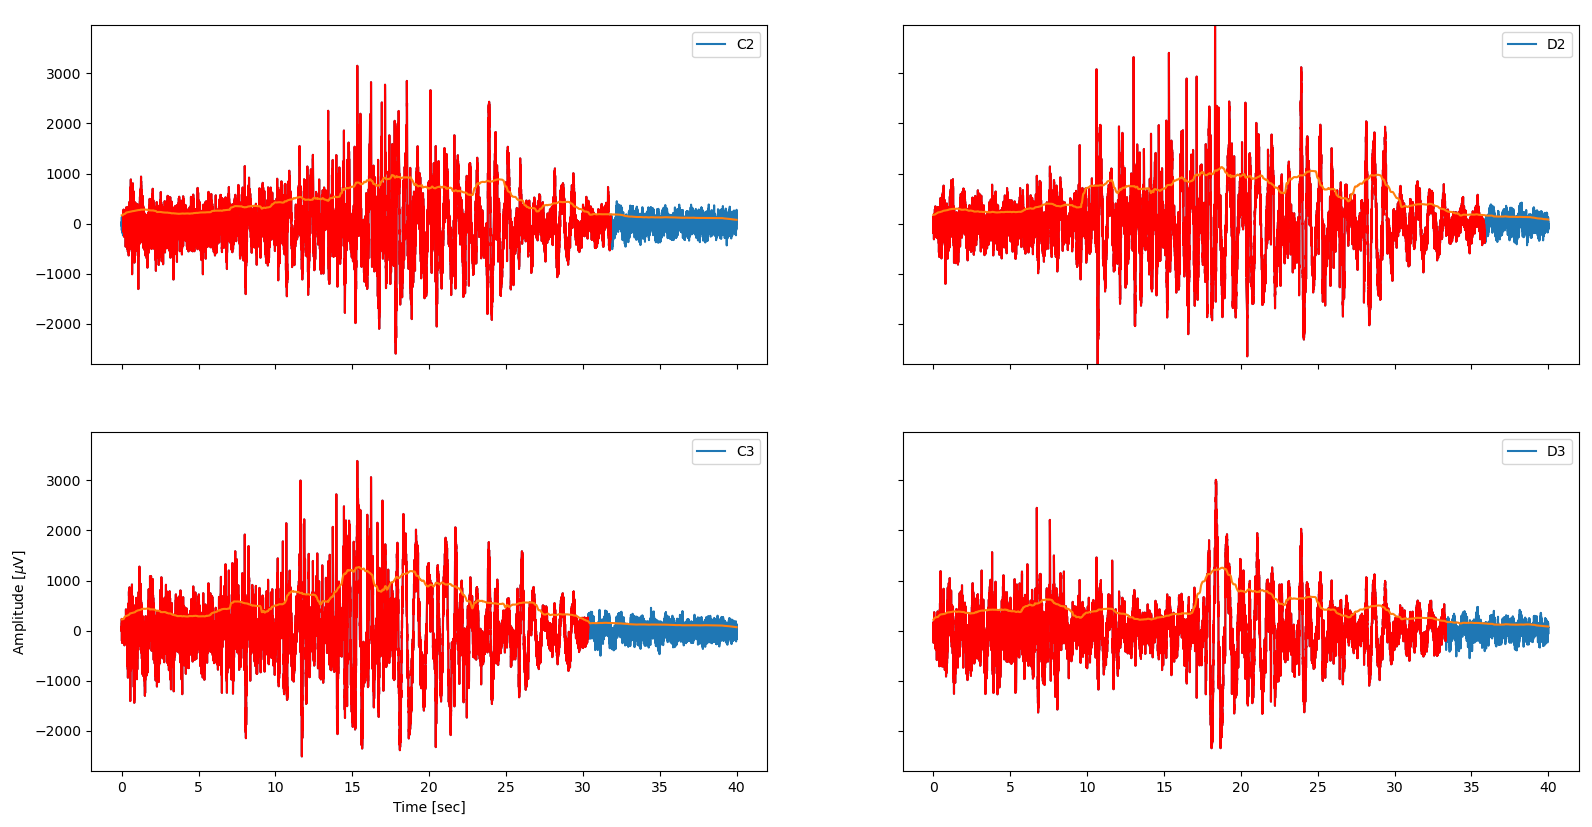
\includegraphics[keepaspectratio,width=\framewidth]{img/4_bursts_std.png}
      \end{center}
      \framebreak
      \begin{center}
       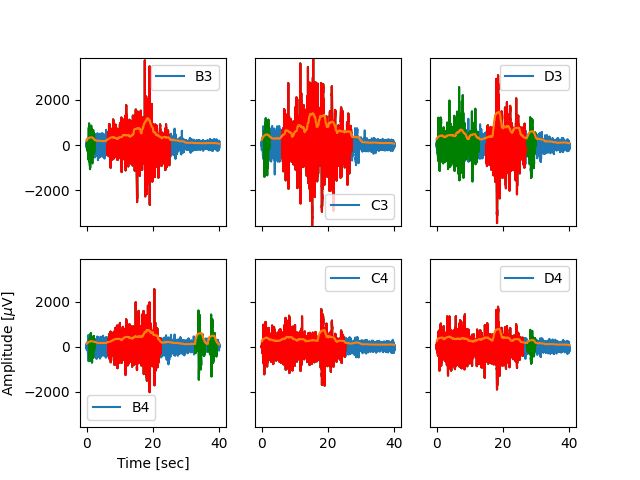
\includegraphics[keepaspectratio,width=\framewidth]{img/bursts_new.png}
      \end{center}
      \framebreak
      
     seizure-like event quantification: \\ 
     \begin{center}
      \hspace*{-1cm}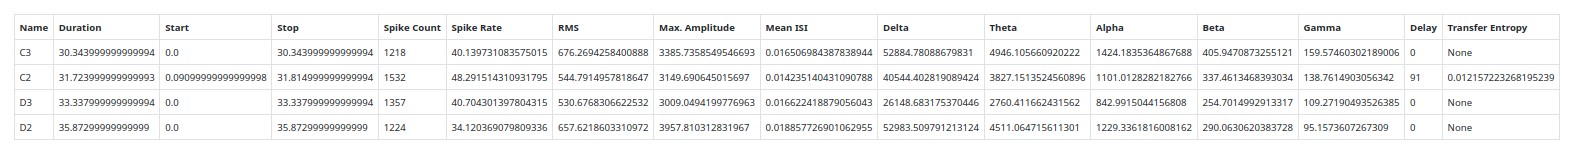
\includegraphics[keepaspectratio,width=1.18\framewidth]{img/4_event_stats_std.png}
     \end{center}
  \end{frame}

\section{The next 6 months (and further)}
\begin{frame}
\begin{center}
 \begin{Huge}
  \textbf{The next 6 months \\(and further)}
 \end{Huge}
 \end{center}
\end{frame}

\begin{frame}{Computing}
\begin{itemize}
  \item batch processing (multiple files/recordings) \\ [2em]
  \item server deployment \\ [2em]
  \item parallelization \\ [2em]
  \item Qt-based GUI?
  \end{itemize}
\end{frame}
  
\begin{frame}{Setup}
  \begin{itemize}
   \item HD/CMOS MEA support \\ [2em]
   \item setup micrograph co-registration \\ [2em]
   \item if $\not\exists$: protocol \& documentation for measurements
  \end{itemize}
\end{frame}

\begin{frame}{Preprocessing}
  \begin{itemize}
   \item Bad channel detection based on SNR, impedances \\ [1em]
   \item (re-) referencing \\ [1em]
   \item between group alignment \\ [1em]
   \item artifact removal using ICA \\ [1em]
   \item epoching \\ [1em]
   \item detrending
  \end{itemize}
\end{frame}

\begin{frame}{Visualization}
 \begin{itemize}
  \item per band power animation \\ [2em]
  \item between group comparisons \\ [2em]
  \item spatial and temporal visualization of analysis
 \end{itemize}

\end{frame}


\begin{frame}[allowframebreaks]{Analysis}
  \begin{itemize}
   \item Per electrode:
  \begin{itemize}
      \item improve peak detection \\ 
      \item improve burst detection \\
      \item FOOOF: periodic \& aperiodic component separation \\
      \item waveform/event sorting, further features \\
      \item waveform \& spike analysis combined \\
      \item spectral (and other kinds of) entropy/complexity meassures \\ [1em]
  \end{itemize}
  \framebreak
  
  \item Between electrodes:
  \begin{itemize}
   \item current source densities \\
   \item transfer entropy/granger causality \\
   \item coherence/``connectivity'' \\
   \item correlation \\
   \item phase-amplitude coupling \\
   \item spontaneous activity
  \end{itemize}
  \framebreak

  \item Within subject: coregistration with atlases \\ $\Rightarrow$ structure-specific comparison
  \item Between subjects: aggregation to group
   \item Group analysis: t-tests, automated listing of significant p-values for the above
  \end{itemize}
\end{frame}

\begin{frame}
 \Huge Famous last words
\end{frame}



\section{References}
    \begin{frame}[allowframebreaks]
      \frametitle{References}
      \begin{tiny}
      \nocite{*}
      \printbibliography
      \end{tiny}
    \end{frame}

 \end{document}
